\section{Jenkins}
\label{sec:jenkins}
    Jenkins byl dřív známý jako Hudson a přejmenoval se po neshodě s Oracle \cite{jenkins-hudson}. Oba projekty pak nějakou dobu byly udržovány souběžně. Oracle svůj systém Hudson oficiálně nikdy nepřestal vyvíjet, ale poslední vydání je ze začátku roku 2016. V následujícím textu se budu věnovat pouze Jenkins, který je dodnes aktivně udržován a má velkou komunitu.

    Hlavní výsadou Jenkins oproti ostatním \CICD systémům je rozšiřitelnost pomocí pluginů.

    \todo{popsat ze jenkins je jenom o pluginech}\blind[1]

    \subsection{Instalace a konfigurace}
        Instalace Jenkins z oficiálního balíčku je přímočařá. Nejprve jsem zaregistroval Jenkins \glstext{APT} repozitář \code{pkg.jenkins.io} a aplikaci nainstaloval. Jenkins ale odmítal nastartovat, protože mu chyběl Java runtime. Očekával bych, že aplikační balíček bude mít nezbytné závislosti minimálně v \textit{suggested packages}. Jenkins v aktuální verzi podporuje pouze Java 8 \cite{jenkins-java}. To je \glstext{TLS} verze z března 2014, která má komerční podporu pouze do ledna 2019 \cite{oracle-eol}.

        Při prvním zobrazení webového rozhraní se provádí konfigurace a volitelná instalace rozšíření. Na rozdíl od např. GitLabu nebo Wordpressu vyžaduje Jenkins výchozí administrátorské heslo, které vygeneroval na disk.

        V roce 2018 přišel Jenkins s možností nahradit ruční klikání konfigurace ve webovém rozhraní kódem (\glstext{CasC}) \cite{jenkins-casc}. Některá klíčová nastavení, konkrétně třeba správa rozšíření, je zatím nestabilní. Dále je nahlášena celá řada nekompatibilit s různými rozšířeními \code{jenkins-casc-compat}.

        Každý projekt je na Jenkins nutné založit a nakonfigurovat ručně. Některá rozšíření tento problém řeší, například \code{GitHub Branch Source Plugin} \cite{jenkins-plugins-gbs} sleduje všechny repozitáře vybraných GitLab uživatelů a pokud v nich najde \code{Jenkinsfile}, založí pro repozitář nový projekt na Jenkins. Původně byly Jenkins projekty konfigurovatelné jenom z webového rozhraní a \glstext{API}. V roce 2014 byla publikován \code{Pipeline Plugin}, který umožňuje popsat konfiguraci projektu skriptem. Na to v roce 2016 navázalo rozšíření \code{Pipeline Model Definition Plugin}, které přináší podporu pro deklarativní popis pipeline, kde Jenkins říkáme co se má stát, ale ne nutně \textit{jak}. Deklarativní pipeline je doporučený způsob nastavení Jenkins projektů \cite{jenkins-best-practices}.

        Problém Jenkins je uživatelské rozhraní. Ve výchozím stavu má \glstext{UI} celou řadu velmi problematických částí: několika-úrovňové menu, které vyžaduje přesný pohyb myší; nesjednocené symboly, navíc často nekonvenční (například modrá koule u úspěšného jobu místo klasické zelené); konfigurace a všechny formuláře jsou složité a běžně obsahují 100+ vstupů. Rozšíření Blue Ocean nabízí alternativní \glstext{UI} pro zobrazení průběhu a výsledků buildů \cite{jenkins-plugin-blueocean}. Bohužel nemodernizuje zbytek Jenkins, administraci. Pokud uživatelé konfigurují projekty výhradně přes \code{Jenkinsfile}, nemusí do původního rozhraní vůbec přistupovat. Osobně mi rozhraní přišlo hezké, ale oproti konkurenčním \CICD pomalé.

    \subsection{Rozšiřitelnost}
        Jenkins má v oficiálním registru přes $1\,500$ rozšíření. Používaných je jich ale jenom zlomek; jak ukazuji \pfxref{na grafu}{fig:jenkins-plugins} často instalovaných rozšíření je jenom kolem $200$. Velmi překvapivé bylo zjištění, že rozšíření jsou často aktualizovaná. \pfxref{Z grafu}{fig:jenkins-plugins-update} lze vidět, že přes $600$ rozšíření mělo vydání v posledním roce.

        \afterpage{
            \begin{figure}[H]
                \centering
                \begin{subfigure}[b]{\textwidth}
                    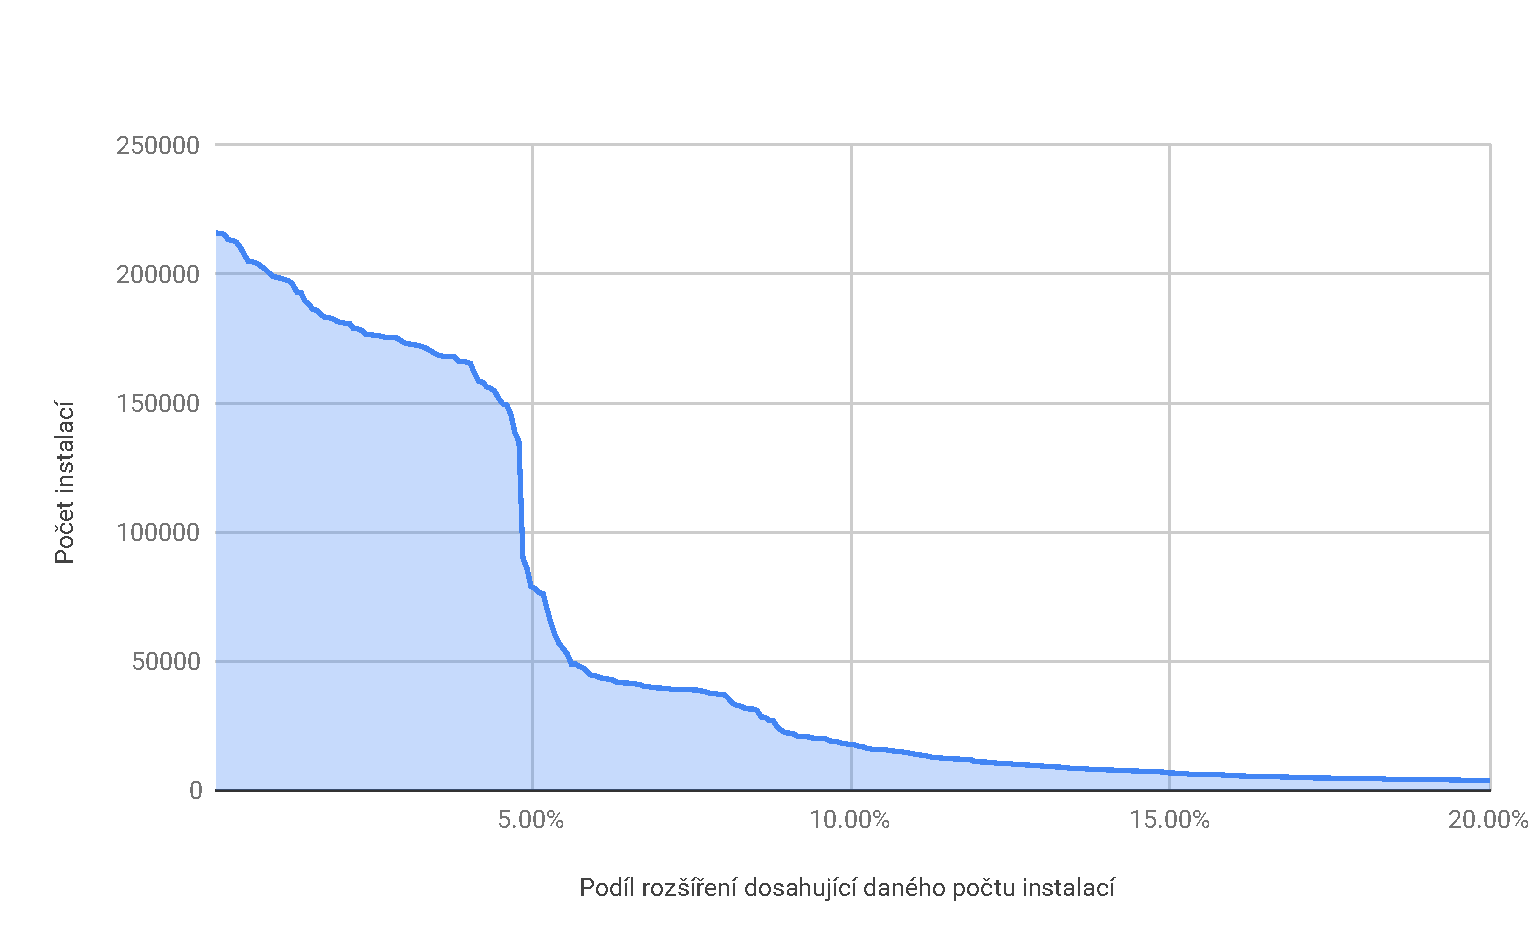
\includegraphics[width=\textwidth,height=9cm,keepaspectratio]{media/jenkins-plugins.pdf}
                    \caption{Rozdělení počtu instalací. Oříznutých 80~\% je klesající dlouhý ocas. Pouze zhruba $80$ rozšíření má víc instalací než $100\,000$. Necelých $200$ rozšíření má víc než $10\,000$ instalací. Přes 60~\% publikovaných rozšíření má méně než $1\,000$ instalací.}
                    \label{fig:jenkins-plugins}
                \end{subfigure}

                \begin{subfigure}[b]{\textwidth}
                    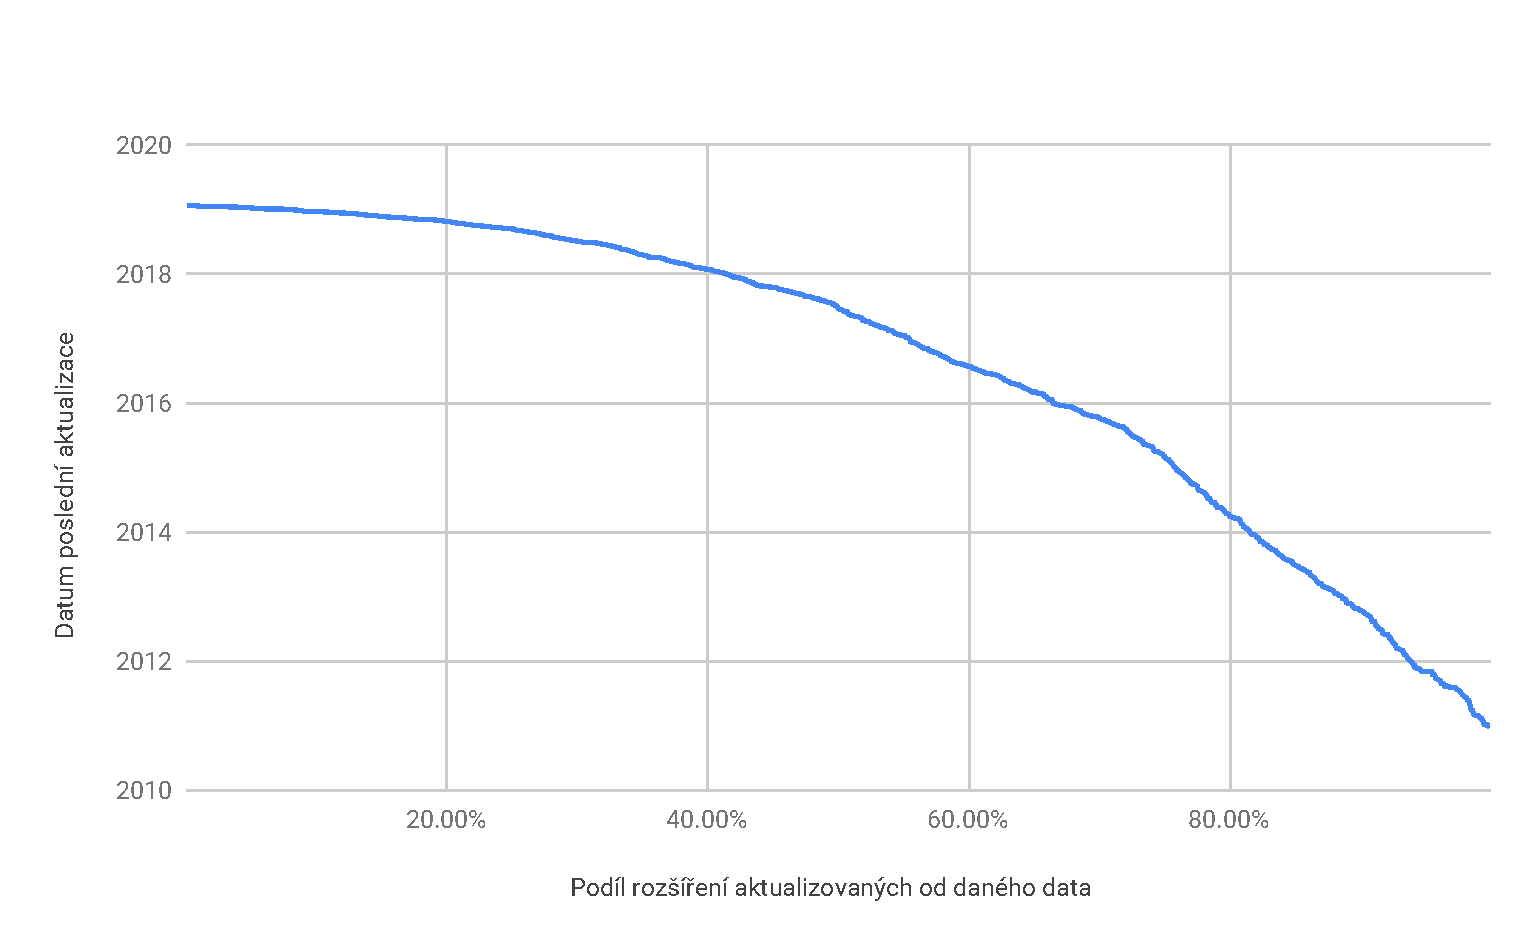
\includegraphics[width=\textwidth,height=9cm,keepaspectratio]{media/jenkins-plugins-update.pdf}
                    \caption{Rozdělení podle poslední aktualizace. Skoro 30~\% byla aktualizována v posledním půl roce. 40~\% rožšíření mělo alespoň jednu aktualizaci za poslední rok.}
                    \label{fig:jenkins-plugins-update}
                \end{subfigure}

                \caption{Zdroj: data vytažena z \url{https://plugins.jenkins.io/}, agregace a vizualizace vlastní. Data jsou dostupná na přiloženém mediu v \code{appendix/jenkins-plugin-*.csv}.}
            \end{figure}
            \clearpage
        }

        \todo{Popsat ekosystem existujich extensions}\blind[1]
        \todo{Popsat moznosti vlastnich rozsireni, groovy atd}\blind[1]

    \subsection{Zabezpečení}
        Stejným způsobem kterým Jenkins deleguje funkcionalitu na pluginy, přenáší zodpovědnost i za bezpečnost. Jádro Jenkins mělo za rok 2018 nahlášeno 53 \glstext{CVE}, rozšíření pro Jenkins skoro 100 \cite{cve-jenkins}.
        \todo{Jaké jsou historická CVE? Jaká je izolace klientů? Co aplikace potřebuje za přístupy?}\blind[3]

        \begin{figure}[hbt]
            \centering
            \makebox[\textwidth][c]{
                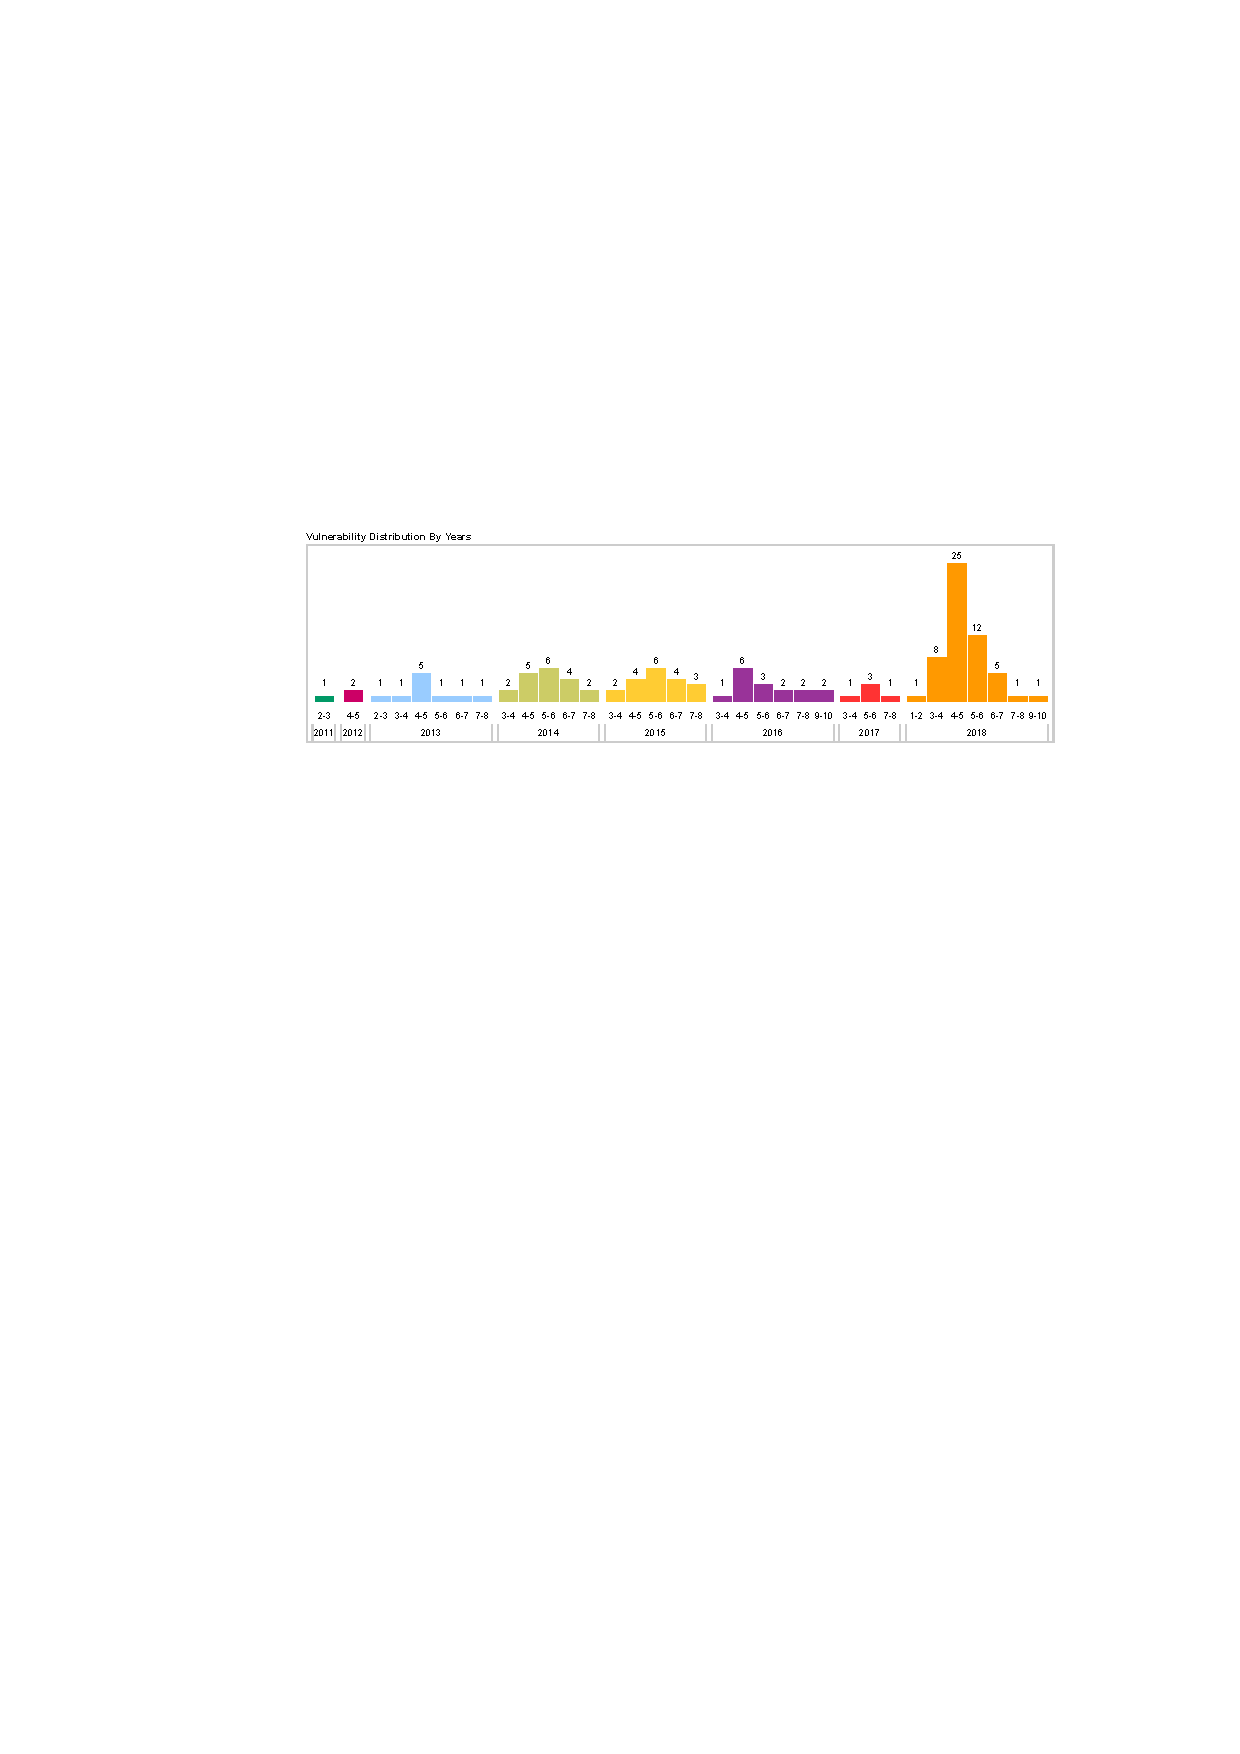
\includegraphics[width=1.2\textwidth]{media/jenkins-cve.pdf}
            }
            \caption{Rozložení Jenkins \glstext{CVE} a přiřazené skóre podle \glstext{CVSS}. Většina nahlášených bezpečnostních chyb bylo \glstext{XSS} a únik informací. Nejvážnější problém v jádru v roce 2018 byla možnost neomezeného spouštění procesů na masteru, které mohl využít každý uživatel s právem přidat nový agent \cite{cve-jenkins}.}
            \label{fig:gitlab-review-cycle}
        \end{figure}

    \subsection{Dostupnost}
        \todo{Při instalaci pluginu to dela restart}
        \todo{Může Jenkins běžet ve víc replikách? Jak se dělá upgrade? Jak stabilní to je?}\blind[3]

    \subsection{Integrace}
        \todo{Integrace Jenkins, oznámení na GitHub/GitLab/Bitbucket/\ldots}\blind[2]
        \todo{Možnosti deploy z Jenkins do cílového systému; k8s, sftp, openstack, \ldots}\blind[5]

    \subsection{Praktické nasazení projektů}
        \subsubsection{Projekt 1}
            \todo{Popsat deploy projektu 1 z Jenkins}\blind[2]
        \subsubsection{Projekt 2}
            \todo{Popsat deploy projektu 2 z Jenkins}\blind[2]
        \subsubsection{Projekt 3}
            \todo{Popsat deploy projektu 3 z Jenkins}\blind[2]
